\chapter{Einleitung}

\paragraph{} Diese Arbeit erläutert die Implementierung einer Seitensuche für die Homepage des \textit{Bielefeld Bioinformatics Service} mit dem Titel \textit{BiBiServSearch}. Eine Seitensuche gehört mittlerweile zu den üblichen Funktionen, die eine Homepage bereitstellen muss und Nutzende haben Erwartungen an Funktionsumfang und Leistungsfähigkeit einer solchen Suche. Vorgestellt wird der Versuch, diesen vielfältigen Anforderungen gerecht zu werden und dabei trotzdem kompatibel mit dem System des \textit{Bielefeld Bioinformatics Service} zu bleiben.
\paragraph{} Im folgenden wird das genaue Ziel und der Kontext der Arbeit vorgestellt. In Kapitel \ref{methoden} sind die theoretischen Grundlagen der Implementierung und in Kapitel \ref{implementierung} die Implementierung selbst beschrieben. Schließlich folgt die Analyse der Ergebnisse der Arbeit in Kapitel \ref{fazit}.

\section{Zielstellung}

\paragraph{} Zur Beschreibung des Problems dieser Arbeit sind zuerst einige Begriffe zu definieren, deren Zusammenhänge auch in einem UML-Domänenmodell im Anhang visualisiert sind (siehe \ref{uml-domain}):
\begin{itemize}
 \item Der \textbf{Suchraum} $\delta$ ist eine Menge von Dokumenten.
 \item Ein \textbf{Dokument} $d$ ist hier lediglich eine geordnete Liste von Vorkommen.
 \item Ein \textbf{Vorkommen} $v$ ist ein Vorkommen eines Wortes (z.B. hat das Wort \textbf{das} in dem Dokument "`Das Schaf sieht das Haus."' zwei Vorkommen).
 \item Ein \textbf{Suchmuster} $p$ ist eine Funktion von Worten in Wahrheitswerte.
 \item Ein \textbf{Match} $m$ für ein Suchmuster $p$ ist ein Wort, für das gilt: $p(w)$ ist wahr.
\end{itemize}

\paragraph{} Dementsprechend lassen sich zwei formale Aufgaben identifizieren:
\begin{enumerate}
 \item Für einen gegebenen Suchraum $\delta$ und ein Suchmuster $p$ alle Vorkommen $v$ zu finden, für die gilt: Das Wort von $v$ ist ein Match für $p$ (\textbf{Suchproblem}).
 \item Für die Ergebnismenge von Vorkommen eine sortierte Liste von Dokumenten erstellen, die wenigstens ein Ergebnisvorkommen enthalten, so dass \textit{das am meisten dem Suchmuster entsprechende Dokument} zuerst genannt ist (\textbf{Sortier- bzw. Scoringproblem}).
\end{enumerate}
 
\paragraph{} Diese sortierte Ergebnisliste ist das, was Nutzenden am Ende eines Suchvorgangs zurückgegeben wird (siehe auch Abbildung \ref{fig-matches-screenshot}). Die Hauptschwierigkeit des Sortierproblems ist dabei nicht, die eigentliche Sortierung der Dokumente vorzunehmen, sondern eine eindeutige Relation zu definieren, nach der die Dokumente sortierbar sind.

\begin{figure}
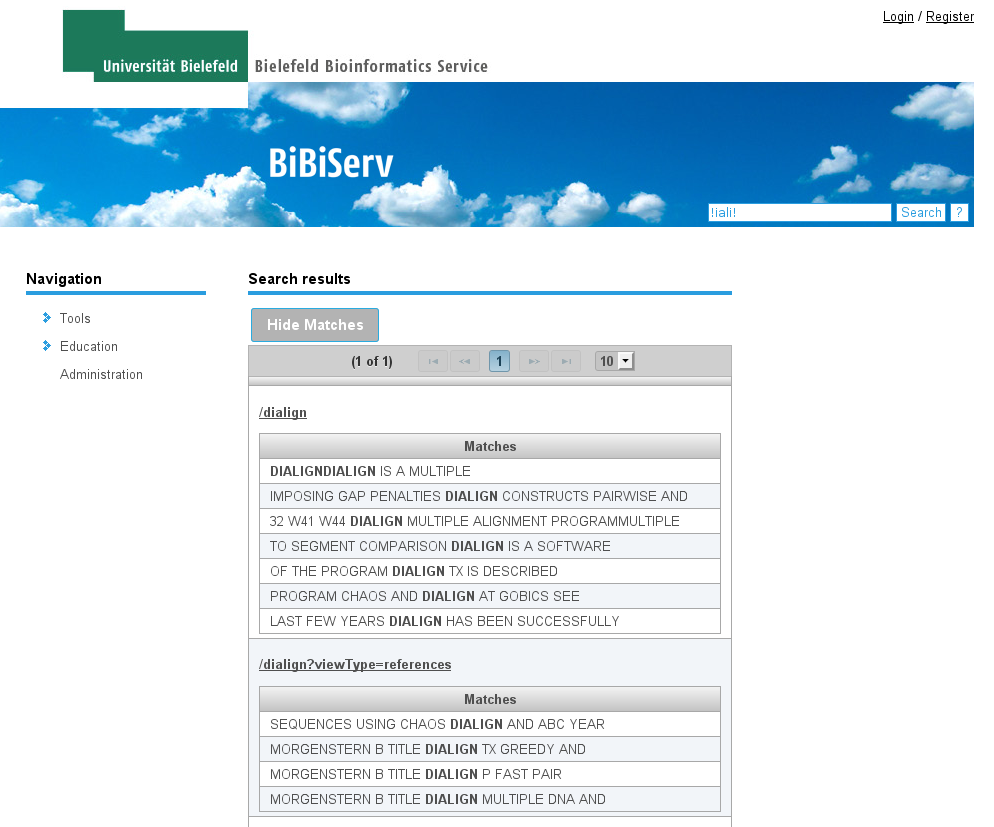
\includegraphics[scale=0.35]{resources/matches_screenshot.png}
\caption{Die Ergebnisseite der Seitensuche für den BiBiServ2. Dargestellt wird eine Liste von Links zu Dokumenten, die Vorkommen von Matches für das Suchmuster enthalten. Die Vorkommen sowie deren benachbarte Worte werden ebenfalls angezeigt.}
\label{fig-matches-screenshot}
\end{figure}

\section{BiBiServ2}

\paragraph{} Der \textit{Bielefeld Bioinformatics Service} ist eine Sammlung bioinformatischer Programme (Tools), die Nutzende aus aller Welt mittels eines Webinterface nutzen können. Der Inhalt des entsprechenden Servers \textit{BiBiServ2} besteht hauptsächlich aus diesen Webinterfaces und zusätzlichen Seiten zu den einzelnen Tools. Diese Seiten werden jedoch nicht händisch erstellt sondern dynamisch aus XML-Beschreibungen der Tools generiert(siehe auch \cite{hagemeier}, S. 5 und S. 29 f.). Dadurch wird die übliche Vorgehensweise, die Menge der HTML-Seiten als Suchraum zu definieren, wenig sinnvoll. Vielmehr besteht der Suchraum aus den Tool-Beschreibungen selbst und den durch die Beschreibungen definierten Resourcen, die auf der Homepage zur Verfügung gestellt werden. Eine Suche auf diesem ungewöhnlichen Suchraum zu ermöglichen ist die hauptsächliche Motivation dieser Arbeit.

\section{Anforderungen}
\label{anforderungen}

\paragraph{} Als Ziel der Implementierung der Suche gilt es, eine Reihe von Anforderungen zu erfüllen. Diese Anforderungen an \textit{BiBiServSearch} lassen sich in verschiedene Kategorien einteilen:

\subsection{Kompatibilität mit dem BiBiServ2}
\label{intro-compatibility}

\paragraph{} Vornehmlich ist es wichtig, dass \textit{BiBiServSearch} im Rahmen des \textit{BiBiServ2} lauffähig ist. Das bedeutet vor allem:
\begin{itemize}
 \item \textit{BiBiServSearch} muss in Java\texttrademark geschrieben sein, um als Teil des bestehenden Client-Server-Systems zu funktionieren und nahtlos in den Ablauf zum Hoch- und Herunterfahren des Servers eingefügt werden zu können.
 \item Das Programm muss XML und alle Dateiformate bearbeiten können, die als Text-Ressourcen von Tools auf dem \textit{BiBiServ2} in Frage kommen (PDF und Reintext).
 \item Die Anwendung muss in der Lage sein, mit einem dynamischen Suchraum umzugehen: Im Rahmen administrativer Zugriffe können Tools auf den Server geladen und wieder entfernt werden. Die Tools und ihre Ressourcen müssen zur Laufzeit auch in den Suchraum eingefügt bzw. daraus gelöscht werden.
\end{itemize}

\subsection{Bedienbarkeit}

\paragraph{} Zur Bedienbarkeit einer Suche tragen vor allem folgende Aspekte bei:
\begin{itemize}
 \item Nutzenden muss eine einfache und verständliche Syntax zum Ausdruck ihrer jeweiligen Suchmuster zur Verfügung gestellt werden. Dabei gilt es, möglichst nicht von den bereits üblichen Standards abzuweichen.
 \item Diese Syntax muss durch eine Hilfeseite erklärt werden.
 \item Die Ergebnisse einer Suche müssen für Nutzende nachvollziehbar sortiert werden: Das erste angezeigte Suchergebnis sollte auch dasjenige sein, dass die/der Nutzende am ehesten \textit{gemeint} hat.
 \item Die Suche sollte fehlertolerant funktionieren: Selbst wenn Nutzende sich vertippen, sollten diejenigen Suchergebnisse zurückgegeben werden, die wahrscheinlich gemeint waren.
\end{itemize}

\subsection{Funktionsumfang}
\label{anforderungen-features}

\paragraph{} In der Regel erwarten Nutzende von einer Seitensuche mehr als die Möglichkeit, einfach nur nach bestimmten Worten suchen zu können und Dokumente als Ergebnis zu erhalten, die genau dieses Wort enthalten. Vielmehr ist das Ziel, folgende Funktionen zu bieten\footnote{Hier wird um der Beispiele willen die fertige Syntax für Suchausdrücke bereits vorweggenommen. Die Syntax ist im Detail in Abschnitt \ref{algo-pattern-language} dokumentiert.}:

\paragraph{}

\begin{tabularx}{\textwidth}{llX}
\hline
\textbf{Suchmodus} & \textbf{Beispielmuster} & \textbf{Beschreibung} \\ [0.1cm]
\hline
Exakte Suche & \texttt{"holder Knabe"} & Suche nach denjenigen Dokumenten, die die Worte "`holder"' und "`Knabe"' in genau dieser Reihenfolge enthalten \\ [0.1cm]
\hline
Teilwortsuche & \texttt{!hold!} & Suche nach allen Dokumenten, die Worte enthalten, für die "`hold"' ein Teilwort ist (z.B. "`Wacholderbeere"') \\ [0.1cm]
\hline
Reguläre Ausdrücke & \texttt{![hg]old!} & Teilwortsuche nach den Worten "`hold"' \underline{und} "`Gold"' (dieses Beispiel erschöpft die Möglichkeiten regulärer Ausdrücke freilich nicht. Mehr darüber ist im Abschnitt \ref{algo-regex} zu lesen.)  \\ [0.1cm]
\hline
Inexakte Suche & \texttt{hold} & Suche nach (Teil-)worten, die dem Wort "`hold"' \textit{hinreichend ähnlich} sind. Dabei meint "`hinreichend ähnlich"' Worte, die Nutzende vielleicht eigentlich meinten, bei denen sie sich aber vertippt haben. Beispielsweise könnte bei der Suchanfrage \texttt{hold} auch "`Gold"' gemeint sein. \\ [0.1cm]
\hline
\end{tabularx}

\paragraph{} Außerdem sollte eine Veränderung des Suchraums durch administrative Anfragen nicht mit Suchanfragen von Nutzenden kollidieren. Hier sind Synchronisationsmechanismen geboten.

\subsection{Effizienzanforderungen}

\paragraph{} In Sachen Effizienz geht es sowohl um Laufzeit- als auch um Speichereffizienz. Bei der Laufzeit haben schnelle Antwortzeiten auf Suchanfragen von Nutzenden die höchste Priorität. Selbst bei schwierigen Suchmustern sollte eine Antwortzeit von maximal 3 Sekunden nicht überschritten werden. Nachrangig ist die Laufzeit bei der Bearbeitung administrativer Anfragen.
\paragraph{} Wesentlich bleibt aber die Speichereffizienz: Eine schnelle Bearbeitung von Suchanfragen erfordert die Repräsentation des Suchraums im Arbeitsspeicher. Da die Bearbeitung von Suchanfragen nicht im eigentlichen Rechengrid des \textit{BiBiServ2} stattfindet, sondern vom Server selbst übernommen wird, steht nur begrenzter Arbeitsspeicher zur Verfügung. Also ist hier eine möglichst speichereffiziente Lösung zu suchen.